\chapter{Implementation}
\label{chap:impl}
\begin{markdown}
  
# Introduction #

This chapter describes the implementation of the GPU support for Julia
presented in this report. The implementation consists of three phases.
__1)__ Creating a LLVM loadable module from a Julia function, __2)__
lowering the function to code executable by a GPU and __3)__ compiling
the code into ptx. The first phase is implemented as in Julia as a
__module generator__, the last two are combined in a __lowering
compiler__.

The CUDA.jl library is used as a glue to transfer data to and from the
device and schedule the generated code on the device.

In this chapter we will iterate through the design. First we look at
the implementation from an overview persepective. Then a simplified
flow through the pipeline. The last section will look at some
importaint details.

# Overview #

\begin{figure}[H]
  \centering
  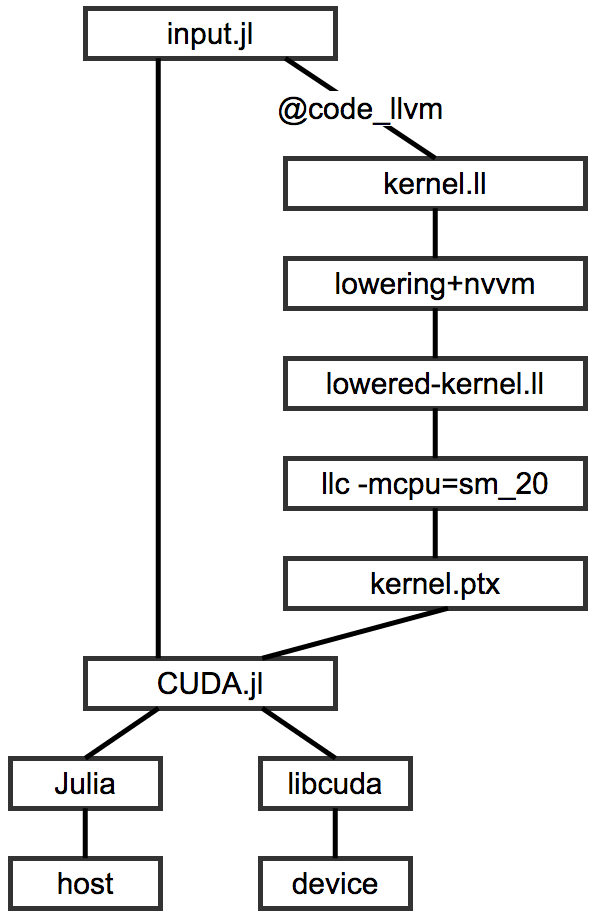
\includegraphics[width=200px]{body/figures/compiler.png}
  \caption{}
  \label{fig:compiler}
\end{figure}

Figure \ref{fig:compiler} illustrates the process of the code
generation. A julia function is turned into LLVM IR with the compiler
builtin macro __@code\_llvm__. This code is then lowered into code
that the LLVM PTX backend can create PTX code for. Here the __llc__
compiler is employed directly without modification. The PTX code can
then be loaded and executed on the GPU with existing CUDA bindings
written for Julia.

## Julia Module Generator ##

The module generator phase is responsible for producing a valid LLVM
__Module__. It is implemented on top of the builtin @code_llvm macro.
The interface to the generator is the __code_module__ function. 

## Lowering Compiler ##

The lowering compiler is built on top of the LLVM static compiler
__llc__. The compiler extends _llc_ by linking to predefined libraries,
a lowering and an annotating compiler pass.

# A Guided tour through the compiler #

This section will go though the compiler step by step looking at the
generated code to show how the code is transformed. Some details are
left out and discussed in Section \ref{sec:implementation-details}
Consider the julia kernel function in figure \ref{fig:julia-copy}.

\begin{figure}[H]
  \begin{minted}{julia}
function copy(from, to)
  i = get_global_id(0);
  to[i] = from[i];

  return
end
  \end{minted}
  \caption{}
  \label{fig:julia-copy}
\end{figure}

## A LLVM module for Julia Function ##

The macro __@code\_llvm__ compiles a julia function with arguments
down to the corresponding LLVM IR representation. In order to load
this string into a LLVM module, function declarations and types used
in the function must be included. As seen in Figure
\ref{fig:copy-llvm} the extra information need is included. 

\begin{figure}[H]
  \begin{minted}{llvm}
%jl_value_t = type { %jl_value_t* }
   
define void @copy(%jl_value_t*, %jl_value_t*) {
top:
  %2 = call i64 @get_global_id(i64 0)
  %3 = call i64 @getindex(%jl_value_t* %0, i64 %2)
  %4 = call i64 @setindex(%jl_value_t* %1, i64 %3, i64 %2)
  ret void
}

declare i64 @setindex(%jl_value_t*, i64, i64)
declare i64 @getindex(%jl_value_t*, i64)
declare i64 @get_global_id(i64)
  \end{minted}
  \caption{}
  \label{fig:copy-llvm}
\end{figure}

## Lowering the code ##

The lowering LLVM pass transforms the function in figure
\ref{fig:copy_llvm} to the one in figure \ref{fig:copy_lowered}. In
this step, the gpu low level implementations for the arrays have been
linked and inlined, in place of the calls to __getindex__ and
__setindex!__ in Figure \ref{fig:copy_llvm}. The __get_global_id__
function has been mangled to enable it to be linked with its
implementation in the next step. The julia arrays represented with
__jl_value_t__ has been replaced with a unboxed integer pointer in the
_global_ address space. The annotating pass has added the
__!nvvm.annontations__ named metadata. An it is set up so the PTX
backend recognizes the function as a kernel.

\begin{figure}[H]
  \begin{minted}{llvm}
target datalayout = "e-p:32:32:32-i1:8:8-i8:8:8- ... -v1024:1024:1024"
target triple = "nvptx64-nvidia-cuda"

declare i64 @get_global_id(i32)

define void @copy(i64 addrspace(1)*, i64 addrspace(1)*) {
top:
  %2 = call i64 @get_global_id(i32 0)
  %3 = getelementptr inbounds i64 addrspace(1)* %0, i64 %2
  %4 = load i64 addrspace(1)* %3, align 8, !tbaa !2
  %5 = getelementptr inbounds i64 addrspace(1)* %1, i64 %2
  store i64 %4, i64 addrspace(1)* %5, align 8, !tbaa !2
  ret void
}

!llvm.ident = !{!0}
!nvvm.annotations = !{!1}

!0 = metadata !{metadata !"Apple LLVM version 6.0 (clang-600.0.54) (based on LLVM 3.5svn)"}
!1 = metadata !{void (i64 addrspace(1)*, i64 addrspace(1)*)* @copy, metadata !"kernel", i32 1}
  \end{minted}
  \caption{}
  \label{fig:julia-copy}
\end{figure}

## Compiling the code to PTX ##

The LLVM static compiler, __llc__, is used to compile the lowered LLVM
IR into PTX code that can be loaded into the GPU. 

## Loading the code into a GPU ##

The last step is done with existing libraries. 

# Implementation details #
\label{sec:implementation-details}

## Disabling inlineing ##

A key to the method presented in this report is the __@noinline__
macro. It is a modification to the Julia compiler. The macro marks a
method so the Julia inlining mechanism will not consider a call to the
method for inlining. 

## Unboxed arrays ##
\label{sec:implementation-details-unboxed}

The unboxed array implementation is a shared implementation between
Julia and OpenCL C. On the Julia side the type is represented by
__GPUVector__. The type is generic and is a Vector of _Int32_,
_Int64_, _Float32_ or _Float64_. The methods for the __setindex!__ and
__getindex__ functions are implement for the Vector type. These are
called when the element operator in Julia is used.

## Function Lowering ##

The kernel function is lowered by substituting a Julia
__GPUVector{T}__ with the LLVM IR __T*__. The replacement starts by
considering the parameters of the kernel. Then the use graph of the
paremeter is considered. 

## Builtin kernel functions ##

As mentioned in Section \ref{} the OpenCL specification defines
builtin functions that are available to a kernel. __libclc__
\cite{libclc} provides an open source implementation of the runtime
library for the LLVM NVPTX backend. This library is used as is and is
linked just before the optimization phase so that the library functions
can be inlined by the LLVM optimizer.

## Supporting multiple primitive types ##

The implementation supports 32- and 64-bits integer and floating point
numbers. To facilitate this the functions mentioned in
\ref{sec:implementation-details-unboxed} are overloaded for the four
types. Type information in Julia is contained inside the argument as a
runtime value. Therefor the information is not accessible by calling
the __@code_llvm__ macro, running at compile time. This is solved by
passing the type information in a named metadata node added to the
module in the module generator. This inplies that the kernel has a fixed
type and must be generated for each type.

\end{markdown}
